%%%% Weekly Report Information %%%%
\newcommand{\handoutName}{Weekly report}
\newcommand{\handoutdate}{Nov 25, 2014}
\newcommand{\duedate}{}
% Header template used for Weekly Reports
\documentclass[11pt,twoside]{article}

\setlength{\oddsidemargin}{0pt}
\setlength{\evensidemargin}{0pt}
\setlength{\textwidth}{6.5in}
\setlength{\topmargin}{0in}
\setlength{\textheight}{8.5in}
\setlength{\voffset}{0in}

\providecommand{\titlesize}{small}


\usepackage{graphicx}
%\usepackage{subfigure}
\usepackage{palatino}
%\usepackage{cmbright}
\newcommand{\myMargin}{1.00in}
%\usepackage[pdftex]{hyperref}
\usepackage[small,bf]{caption}
\usepackage{amsmath}
\usepackage[usenames,dvipsnames]{color}
\usepackage{fancyhdr}
\pagestyle{fancy}
\usepackage{datetime}
\usepackage{fancyvrb}
\usepackage{color}
\usepackage[\titlesize, compact]{titlesec}
\usepackage{multicol}
\usepackage{enumitem}
\usepackage{pdfpages}
\usepackage{mdwlist}


\usepackage[ruled]{algorithm}
\usepackage{algpseudocode}

\usepackage{caption}
\usepackage{subcaption}



\newdateformat{dashdate}{\THEYEAR-\twodigit{\THEMONTH}-\twodigit{\THEDAY}}
\def\Tiny{\fontsize{3pt}{3pt}\selectfont}

\providecommand{\handoutName}{Handout title}
\providecommand{\handoutdate}{Handout date}
\providecommand{\duedate}{}

\lhead{Meeting with Prof. Becker\\
Fall, 2014}
\chead{}
\rhead{ Shiva Shahrokhi\\
\handoutdate }
\lfoot{}
\cfoot{\thepage}
\rfoot{\dashdate \Tiny \textcolor{Gray}{\today}}
\renewcommand{\headrulewidth}{0.4pt}
\renewcommand{\footrulewidth}{0.4pt}

\begin{document}

\vspace{0.60in}
\begin{center}
{\Large\textbf{\handoutName}}\\
\vspace{0.03in}
\textbf{\duedate}\\
\end{center}

\newcommand{\todo}[1]{
  \textcolor{Red}{
    \begin{tabular}{|c|}
      \hline
      \em \large \bfseries todo: \normalfont \normalsize #1 \\
      \hline
    \end{tabular}}
}


\section{My \emph{Objectives} this week}
\begin{itemize}
\item Plotting all the plots with MATLAB better and put them all in the same picture.
\item Write a Code to Control Variance.
\end{itemize}


\section{My \emph{Accomplishments} this week}

\subsection{\emph{Auto Controllers}}

\begin{itemize}
\item different gain values.
\end{itemize}




\begin{figure}
        \centering
        \begin{subfigure}[b]{0.3\textwidth}
                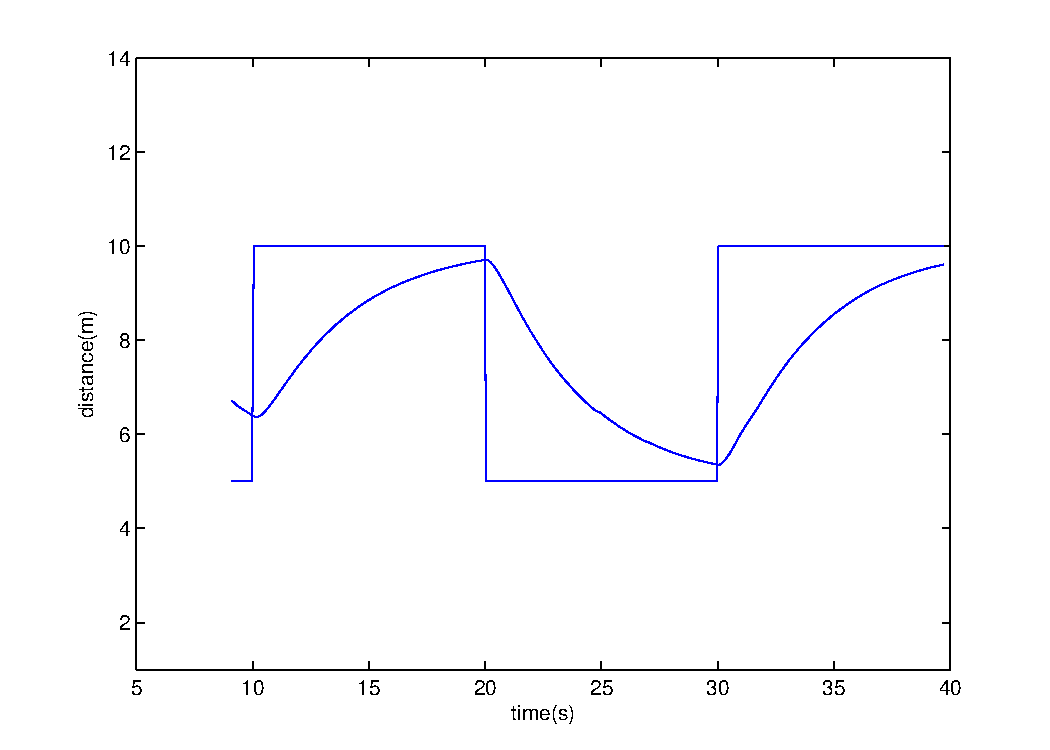
\includegraphics[width=\textwidth]{fig/gain1d1.pdf}
                \caption{g 1, d 1}
                \label{fig:gull}
        \end{subfigure}%
        ~ %add desired spacing between images, e. g. ~, \quad, \qquad, \hfill etc.
          %(or a blank line to force the subfigure onto a new line)
        \begin{subfigure}[b]{0.3\textwidth}
                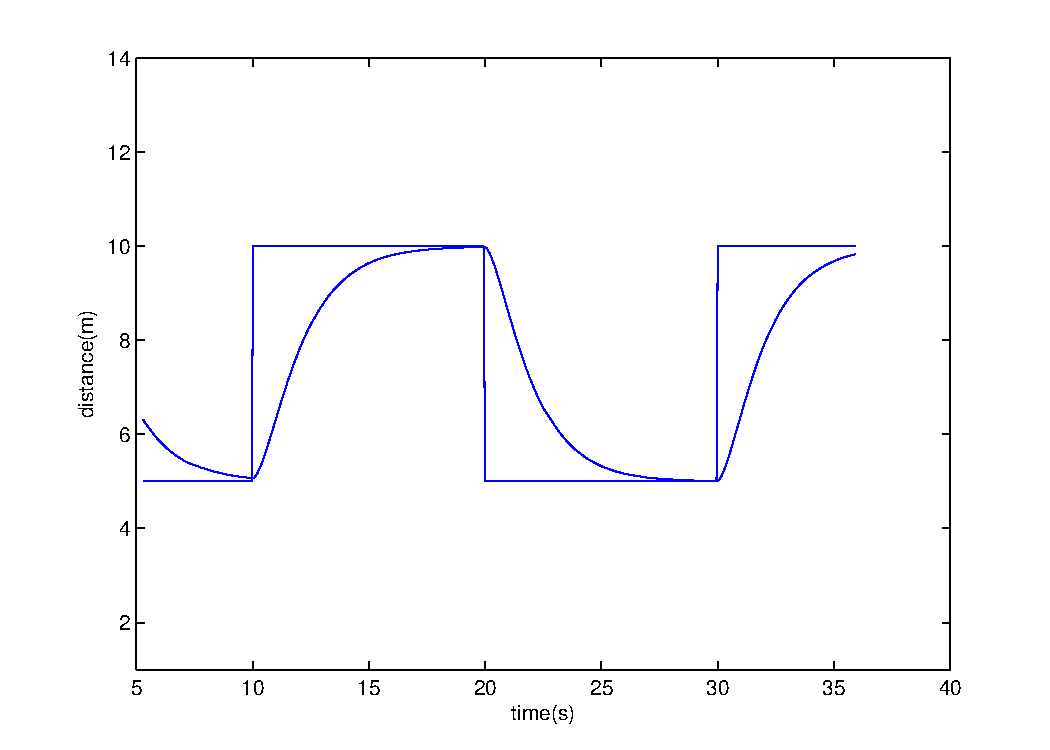
\includegraphics[width=\textwidth]{fig/gain2d1.pdf}
                \caption{g 2, d 1}
                \label{fig:tiger}
        \end{subfigure}
        ~ %add desired spacing between images, e. g. ~, \quad, \qquad, \hfill etc.
          %(or a blank line to force the subfigure onto a new line)
        \begin{subfigure}[b]{0.3\textwidth}
                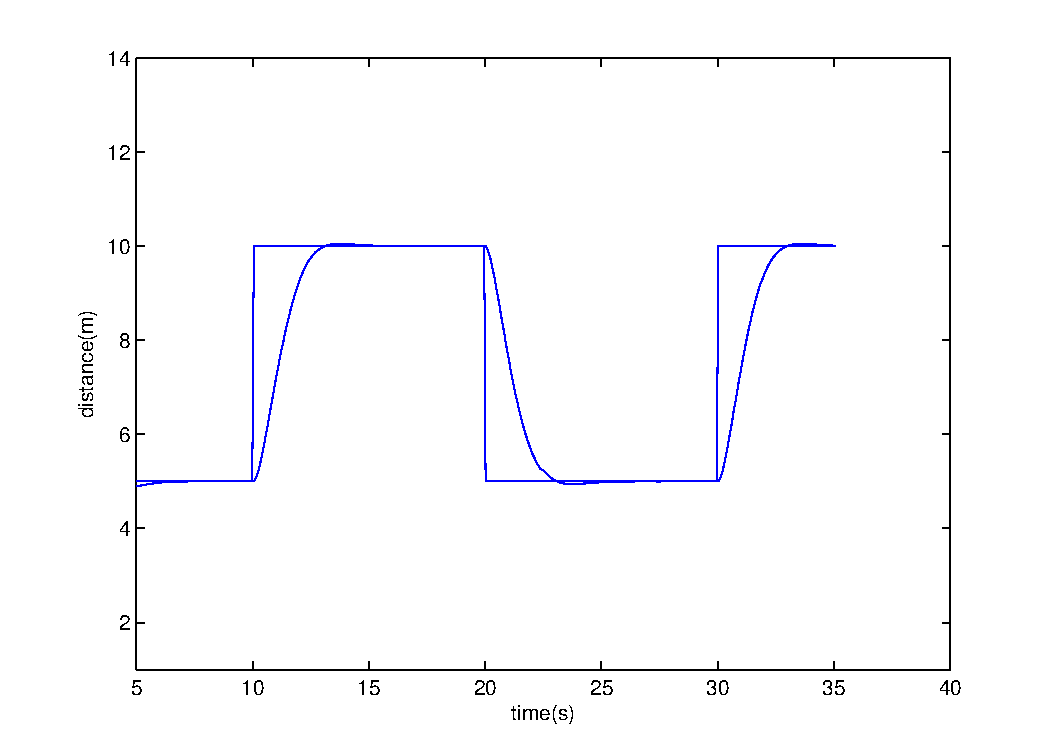
\includegraphics[width=\textwidth]{fig/gain4d1.pdf}
                \caption{g 4, d 1}
                \label{fig:mouse}
        \end{subfigure}
                \begin{subfigure}[b]{0.3\textwidth}
                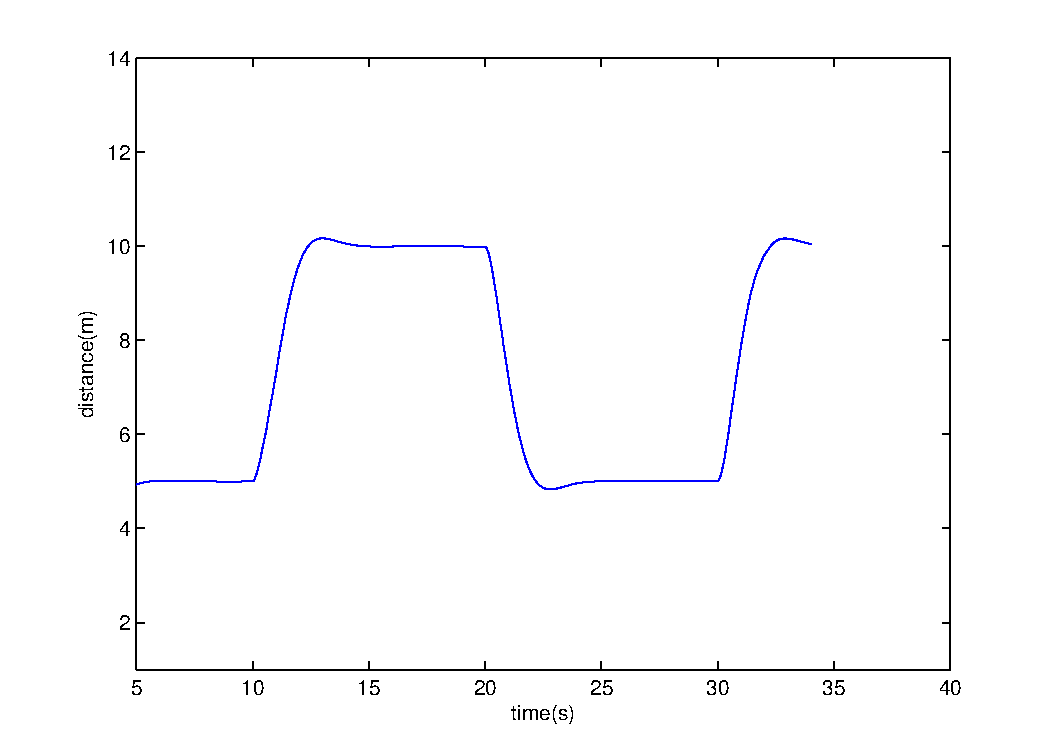
\includegraphics[width=\textwidth]{fig/gain5d1.pdf}
                \caption{g 5, d 1}
                \label{fig:gull}
        \end{subfigure}%
        ~ %add desired spacing between images, e. g. ~, \quad, \qquad, \hfill etc.
          %(or a blank line to force the subfigure onto a new line)
        \begin{subfigure}[b]{0.3\textwidth}
                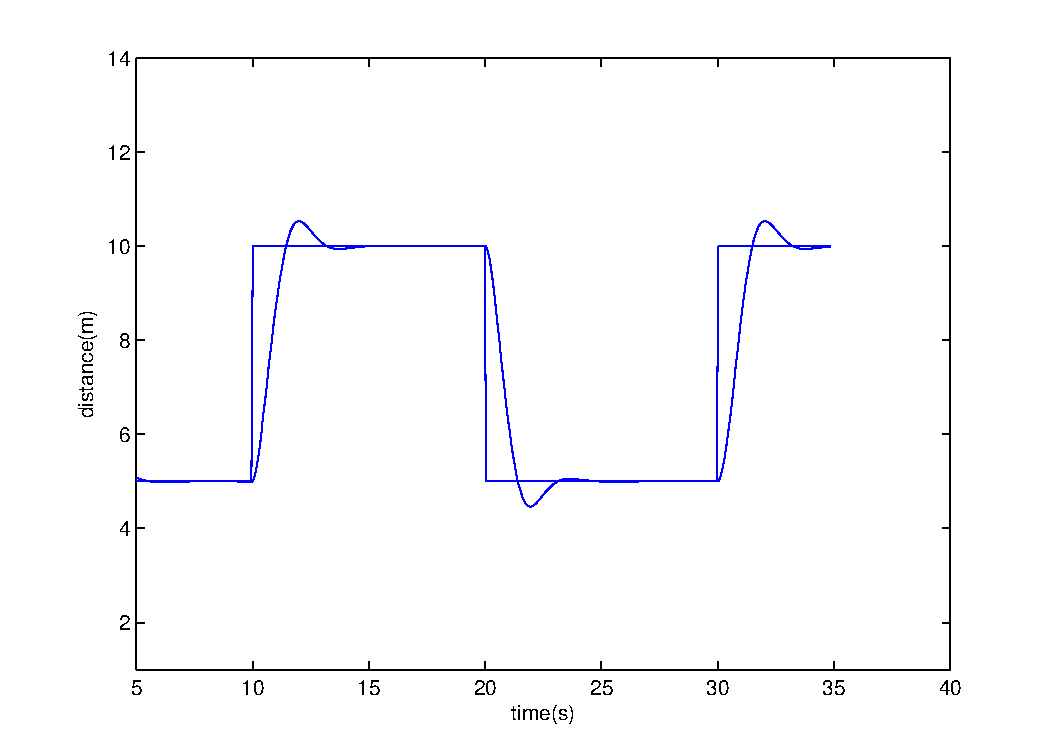
\includegraphics[width=\textwidth]{fig/gain8d1.pdf}
                \caption{g 8, d 1}
                \label{fig:tiger}
        \end{subfigure}
        ~ %add desired spacing between images, e. g. ~, \quad, \qquad, \hfill etc.
          %(or a blank line to force the subfigure onto a new line)
        \begin{subfigure}[b]{0.3\textwidth}
                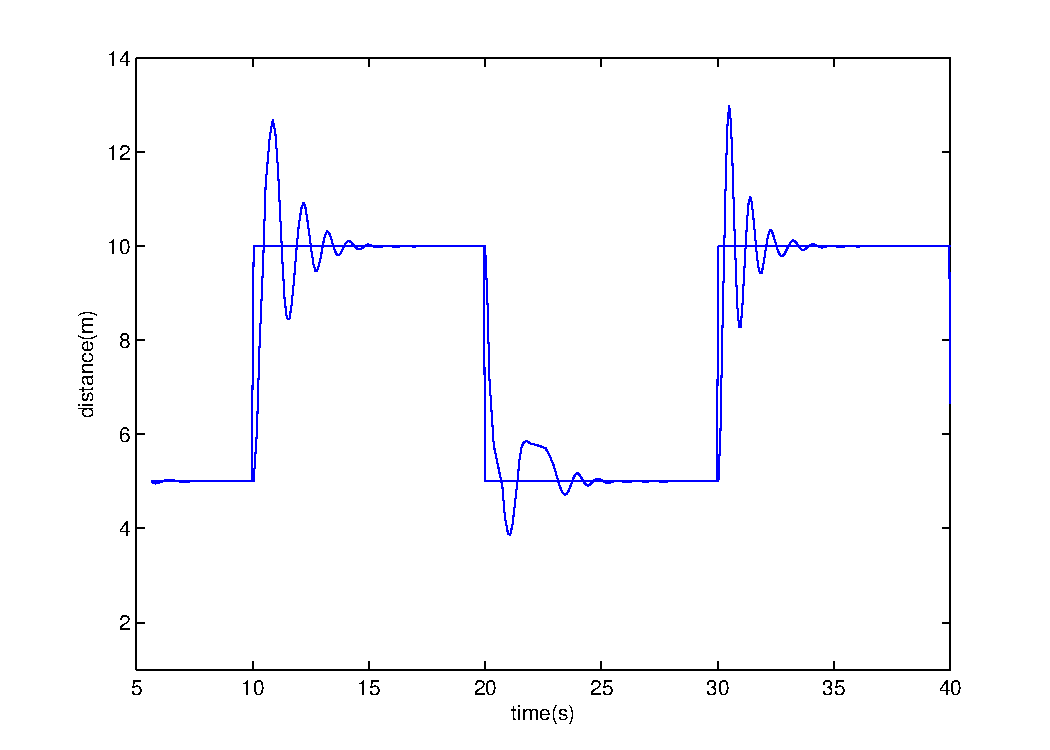
\includegraphics[width=\textwidth]{fig/gain100d1.pdf}
                \caption{g 100, d 1}
                \label{fig:mouse}
        \end{subfigure}
        \caption{Different Gain Values}\label{fig:animals}
\end{figure}



I tested 20 trials to find the best kgain. And I found out that for the derivative of 1, the best gain value is 4.

\begin{itemize}
\item different gain derivatives. I tested with the gain value of 4:
\end{itemize}

\begin{figure}
        \centering
        \begin{subfigure}[b]{0.3\textwidth}
                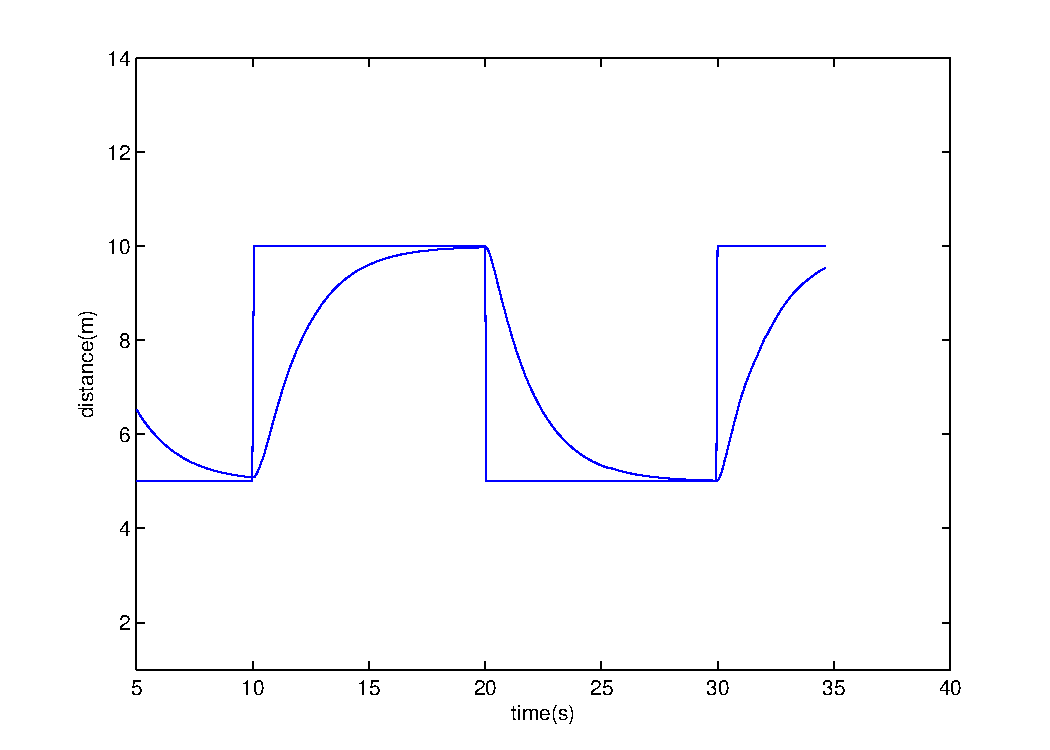
\includegraphics[width=\textwidth]{fig/gain4d2.pdf}
                \caption{g 4, d 2}
                \label{fig:gull}
        \end{subfigure}%
        ~ %add desired spacing between images, e. g. ~, \quad, \qquad, \hfill etc.
          %(or a blank line to force the subfigure onto a new line)
        \begin{subfigure}[b]{0.3\textwidth}
                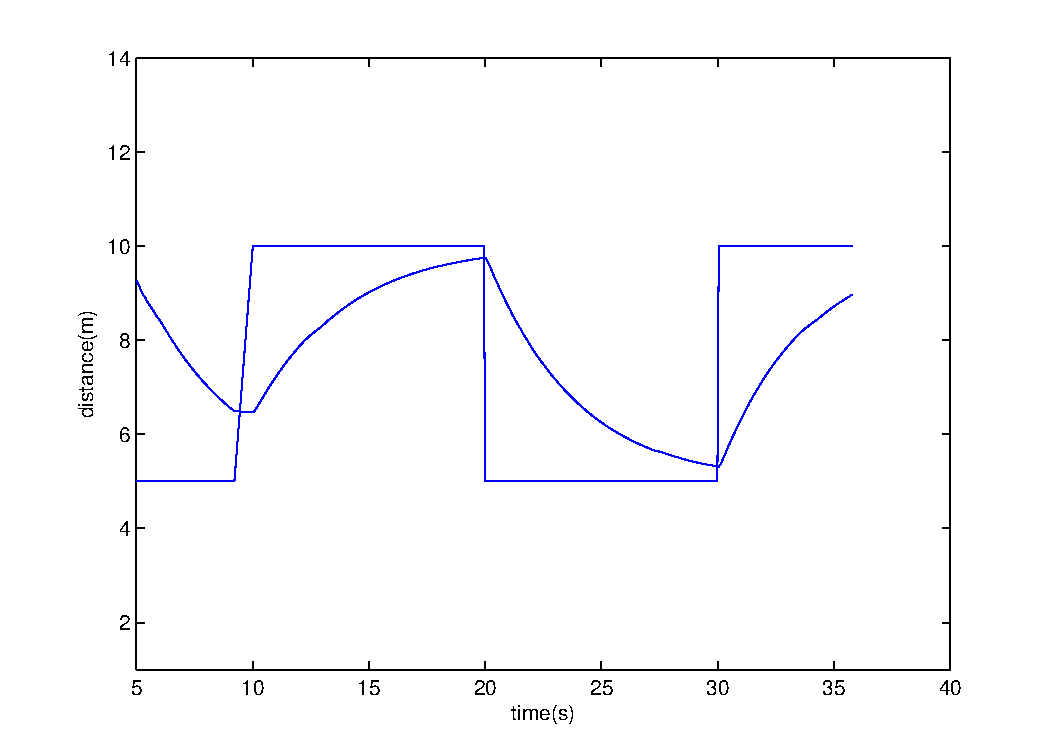
\includegraphics[width=\textwidth]{fig/gain4d4.pdf}
                \caption{g 4, d 4}
                \label{fig:tiger}
        \end{subfigure}
        ~ %add desired spacing between images, e. g. ~, \quad, \qquad, \hfill etc.
          %(or a blank line to force the subfigure onto a new line)
        \begin{subfigure}[b]{0.3\textwidth}
                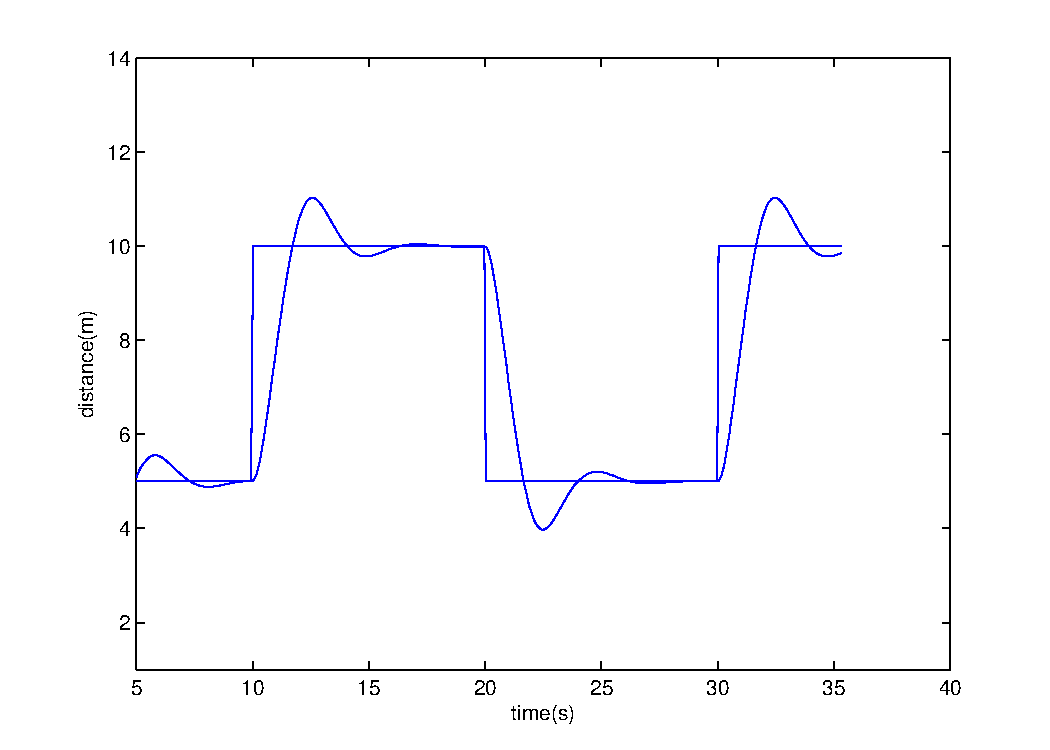
\includegraphics[width=\textwidth]{fig/gain4d05.pdf}
                \caption{g 4, d 0.5}
                \label{fig:mouse}
        \end{subfigure}
         \caption{Different Derivative Values}\label{fig:animals}
\end{figure}

It shows that for the gain value 4, the best derivative is 1.

\begin{itemize}
\item Write a code to control variance.
\end{itemize}

I wrote a code that goes to corner when we want to make variance lower, and goes to center when we want to make variance higher.


\section{My \emph{Plan} for next week}

\begin{itemize}
\item Applying variance and covariance and standard deviation. 
\item Which one of them is the best?
\end{itemize}

\subsection{Meeting with Dr. Becker On Wednesday 19th, 1 pm }

\begin{itemize}
\item Deciding what to take for the next semester
\item What to survey for lab access
\item Show him results.
\end{itemize}

\end{document}
